\chapter{The Epsilon Model Connectivity Layer (EMC)}
\label{sec:Design.EMC}

This section discusses the design of the Epsilon Model Connectivity (EMC) layer. EMC provides abstraction facilities over concrete modelling technologies such as EMF, XML etc. and enables Epsilon programs to interact with models conforming to these technologies in a uniform manner. A graphical overview of the design is displayed in Figure \ref{fig:EMC}.

%\begin{landscape}

\begin{sidewaysfigure}
	\centering
		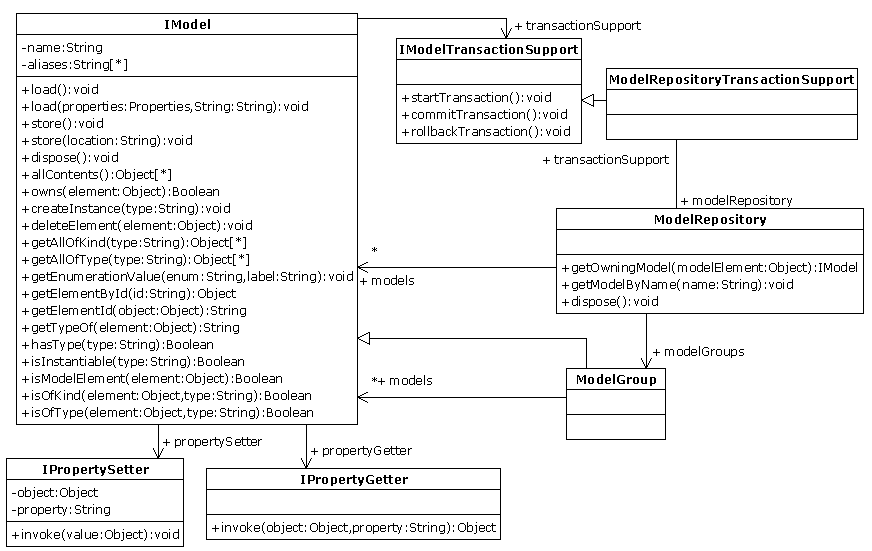
\includegraphics{images/EMC.png}
	\caption{Overview of the Epsilon Model Connectivity layer}
	\label{fig:EMC}
\end{sidewaysfigure}

%\end{landscape}

To abstract away from diverse model representations and APIs provided by different modelling technologies, EMC defines the \emph{IModel} interface. \emph{IModel} provides a number of methods that enable querying and modifying the model elements it contains at a higher level of abstraction. To enable languages and tools that build atop EMC to manage multiple models simultaneously, the \emph{ModelRepository} class acts as a container that offers fa\c{c}ade services. The following sections discuss these two core concepts in detail.

\section{The IModel interface}

Each model specifies a name which must be unique in the context of the model repository in which it is contained. Also, it defines a number of aliases; that is non-unique alternate names; via which it can be accessed. The interface also defines the following services.

\section{Loading and Persistence}

The \emph{load()} and \emph{load(properties : Properties)} methods enable extenders to specify in a uniform way how a model is loaded into memory from the physical location in which it resides. Similarly, the \emph{store()} and \emph{store(location : String)} methods are used to define how the model can be persisted from memory to a permanent storage location.

\section{Type-related Services}

The majority of metamodelling architectures support inheritance between meta-classes and therefore two types of type-conformance relationships generally appear between model elements and types. The \emph{type-of} relationship appears when a model element is an instance of the type and the \emph{kind-of} relationship appears when the model element is an instance of the type or any of its sub-types. Under this definition, the \emph{getAllOfType( type : String )} and the \emph{getAllOfKind( type : String )} operations return all the elements in the model that have a type-of and a kind-of relationship with the type in question respectively.

Similarly, the \emph{isTypeOf( element : Object, type : String )} and \emph{isKindOf( element : Object, type : String)} return whether the element in question has a type-of or a kind-of relationship with the type respectively. The \emph{getTypeOf( element : Object )} method returns the fully-qualified name of the type an element conforms to.

The \emph{hasType( type : String )} method returns true if the model supports a type with the specified name. To support technologies that enable users to define abstract (non-instantiable) types, the \emph{isInstantiable( type : String )} method returns if instances of the type can be created.

\section{Ownership}

The \emph{allContents()} method returns all the elements that the model contains and the \emph{owns( element : Object )} method returns true if the element under question belongs to the model.

\section{Creation, Deletion and Modifications}
\label{sec:Design.EMC.CRUD}

Model elements are created and deleted using the \emph{createInstance( type : String )} and \emph{deleteElement( element : Object )} methods respectively.

To retrieve and set the values of properties of its model elements, \emph{IModel} uses its associated \emph{propertyGetter} (\emph{IPropertyGetter}) and \emph{propertySetter} (\emph{IPropertySetter}) respectively. Technology-specific implementations of those two interfaces are responsible for accessing and modifying the value of a property of a model element through their \emph{invoke( element : Object, property : String)} and \emph{invoke( value : Object )} respectively.

\section{The IModelTransactionSupport interface}
\label{sec:EMC.ModelTransactionSupport}
In its \emph{transactionSupport} property, a model can optionally (if the target modelling technology supports transactions) specify an instance of an implementation of the \emph{IModelTransactionSupport} interface. The interface provides transaction-related services for the specific modelling technology. The interface provides the \emph{startTransaction()}, \emph{commitTransaction()} and \emph{rollbackTransaction()} methods that start a new transaction, commit and roll back the current transaction respectively.

\section{The ModelRepository class}

A model repository acts as a container for a set of models that need to be managed in the context of a task or a set of tasks. Apart from a reference to the models it contains, \emph{ModelRepository} also provides the following fa\c{c}ade functionality.

The \emph{getOwningModel( element : Object )} method returns the model that owns a particular element. The \emph{transactionSupport} property specifies an instance of the \emph{ModelRepositoryTransactionSupport} class which is responsible for aggregate management of transactions by delegating calls to its \emph{startTransaction()}, \emph{commitTransaction()} and \emph{abortTransaction()} methods, to the respective methods of instances of \emph{IModelTransactionSupport} associated with models contained in the repository.

\section{The ModelGroup class}

A \emph{ModelGroup} is a group of models that have a common alias. \emph{ModelGroups} are calculated dynamically by the model repository based on common model aliases. That is, if two or more models share a common alias, the repository forms a new model group. Since \emph{ModelGroup} implements the \emph{IModel} interface, clients can use all the methods of \emph{IModel} to perform aggregate operations on multiple models, such as collecting the contents of more than one models. An exception to that is the \emph{createInstance( type : String )} method which cannot be defined for a group of models as it cannot be determined in which model of the group the newly created element should belong.

\section{Assumptions about the underlying modelling technologies}

The discussion provided above has demonstrated that EMC makes only minimal assumptions about the structure and the organization of the underlying modelling technologies. Thus, it intentionally refrains from defining classes for concepts such as \emph{model element}, \emph{type} and \emph{metamodel}. By contrast, it employs a lightweight approach that uses primitive strings for type names and objects of the target implementation platforms as  model elements. There are two reasons for this decision.

The primary reason is that by minimizing the assumptions about the underlying technologies EMC becomes more resistant to future changes of the implementations of the current technologies and can also embrace new technologies without changes.

Another reason is that if a heavy-weight approach was used, extending the platform with support for a new modelling technology would involve providing wrapping objects for the native objects which represent model elements and types in the specific modelling technology. Experiments in the early phases of the design of EMC demonstrated that such a heavy-weight approach significantly increases the amount of memory required to represent the models in memory, degrades performance and provides little benefits in reward\footnote{Recent developments in the context of the ATL transformation language have also demonstrated significant performance gains delivered by using native model element representations. Relevant benchmarks can be found \url{http://wiki.eclipse.org/ATL_VM_Testing}}.

